\begin{figure}
	\centering
	
	\begin{minipage}{0.27\linewidth}
		\center \scriptsize
		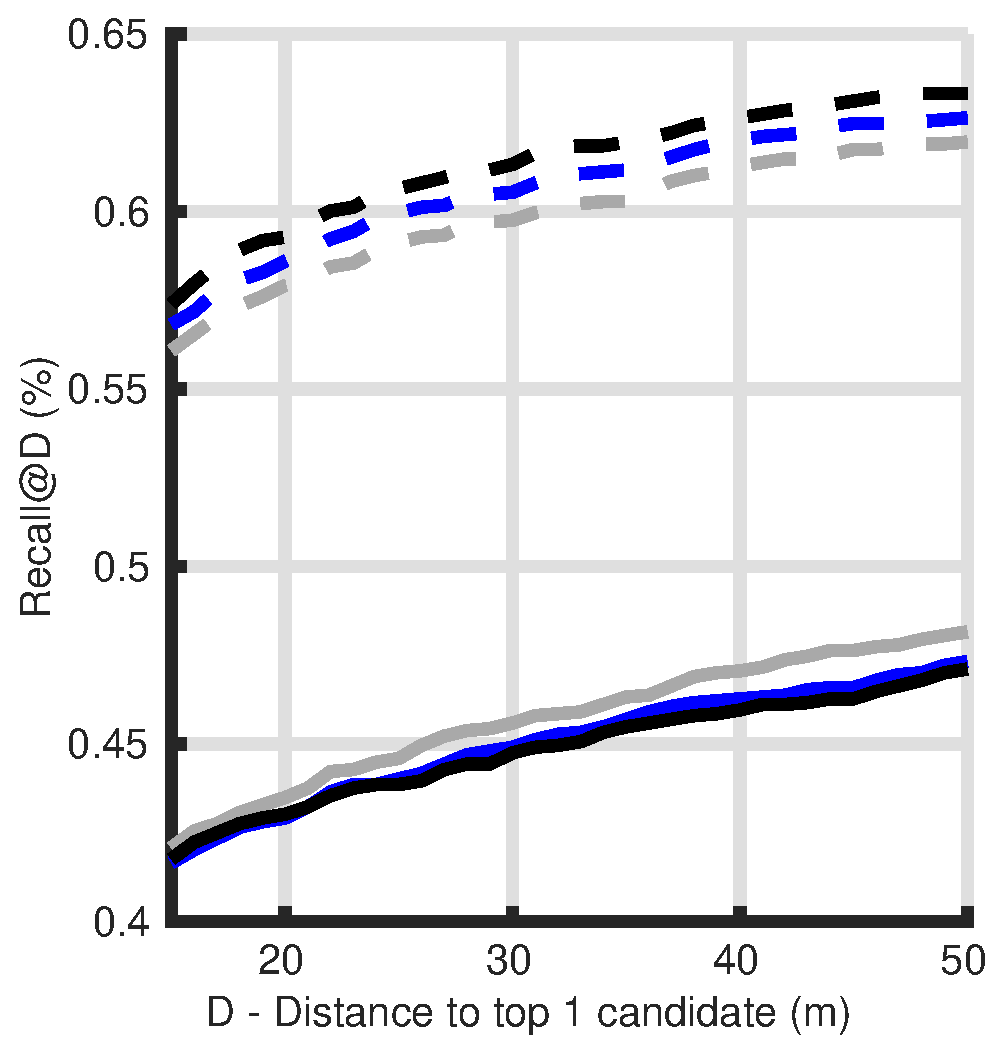
\includegraphics[width=\linewidth]{plot/depth_vs_ref/Results_cmu_lt/distance}	
		
		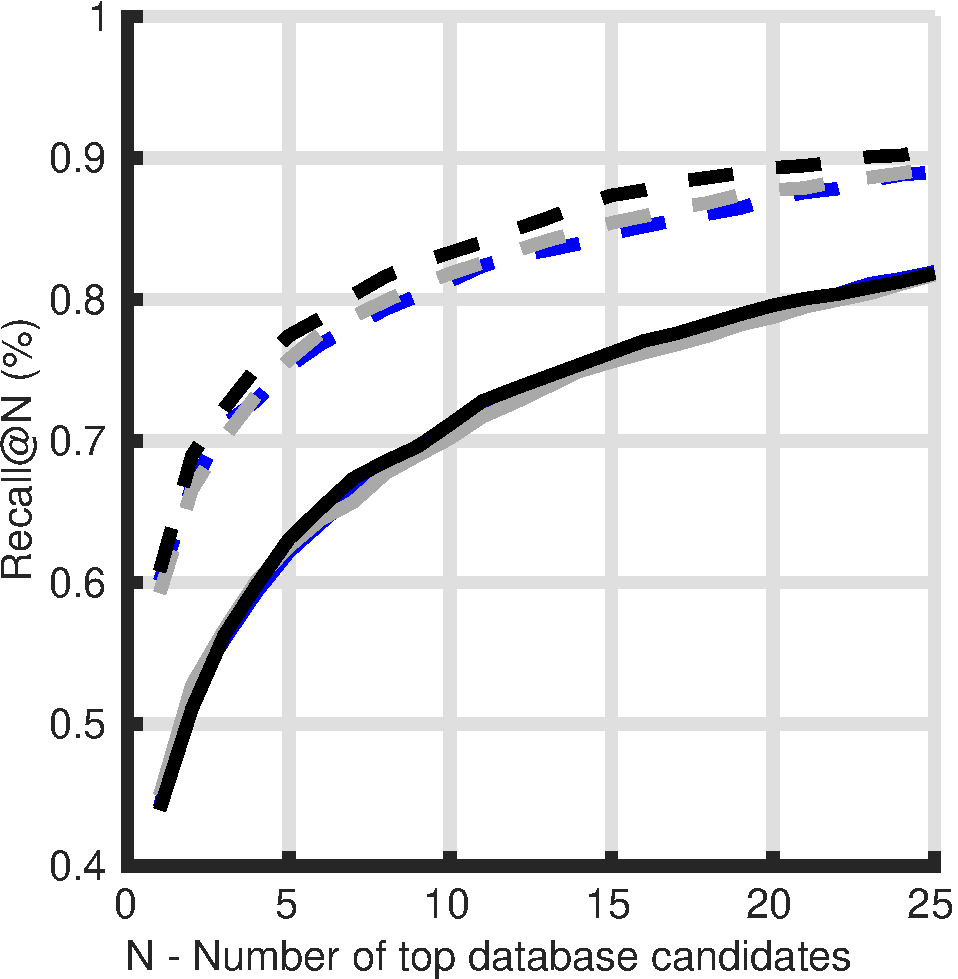
\includegraphics[width=\linewidth]{plot/depth_vs_ref/Results_cmu_lt/recall}
		
		c) CMU -- LT
	\end{minipage}
	\begin{minipage}{0.27\linewidth}
		\center \scriptsize
		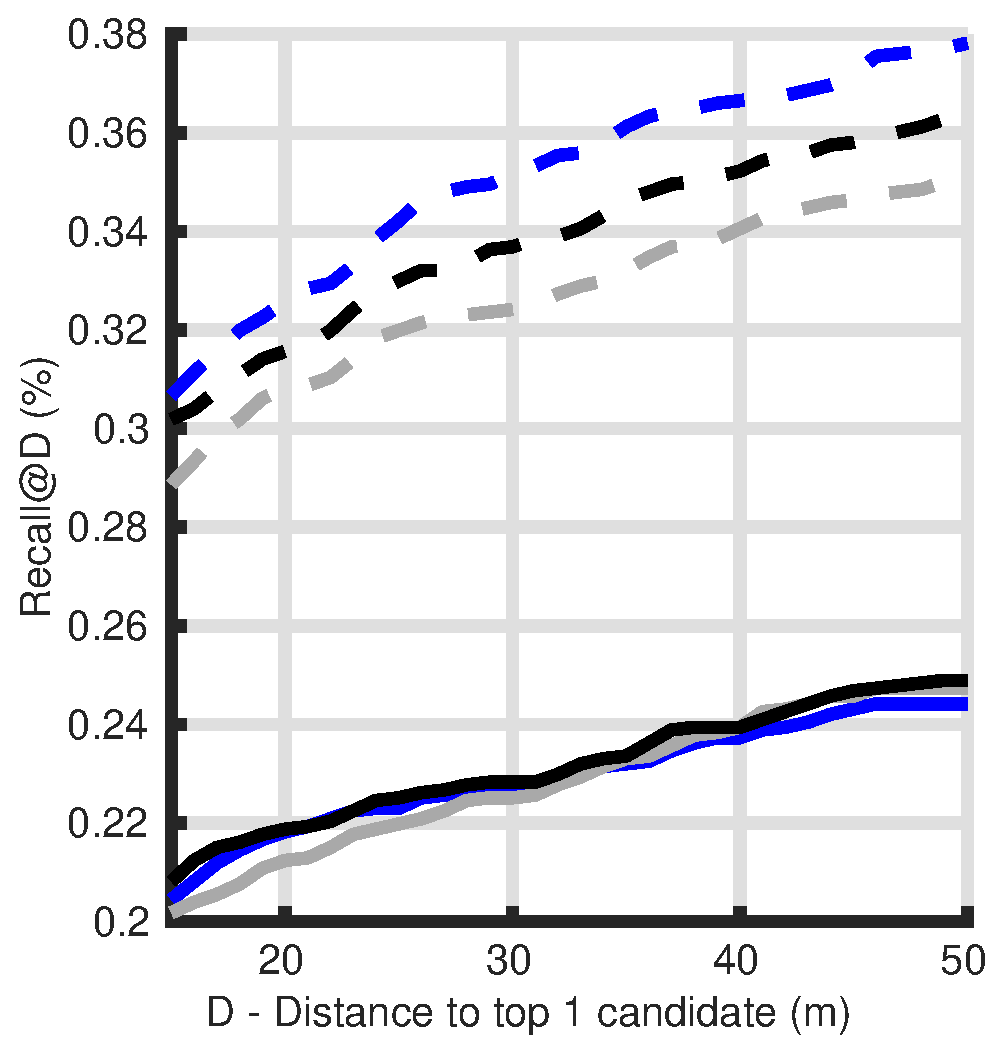
\includegraphics[width=\linewidth]{plot/depth_vs_ref/Results_cmu_snow/distance}	
		
		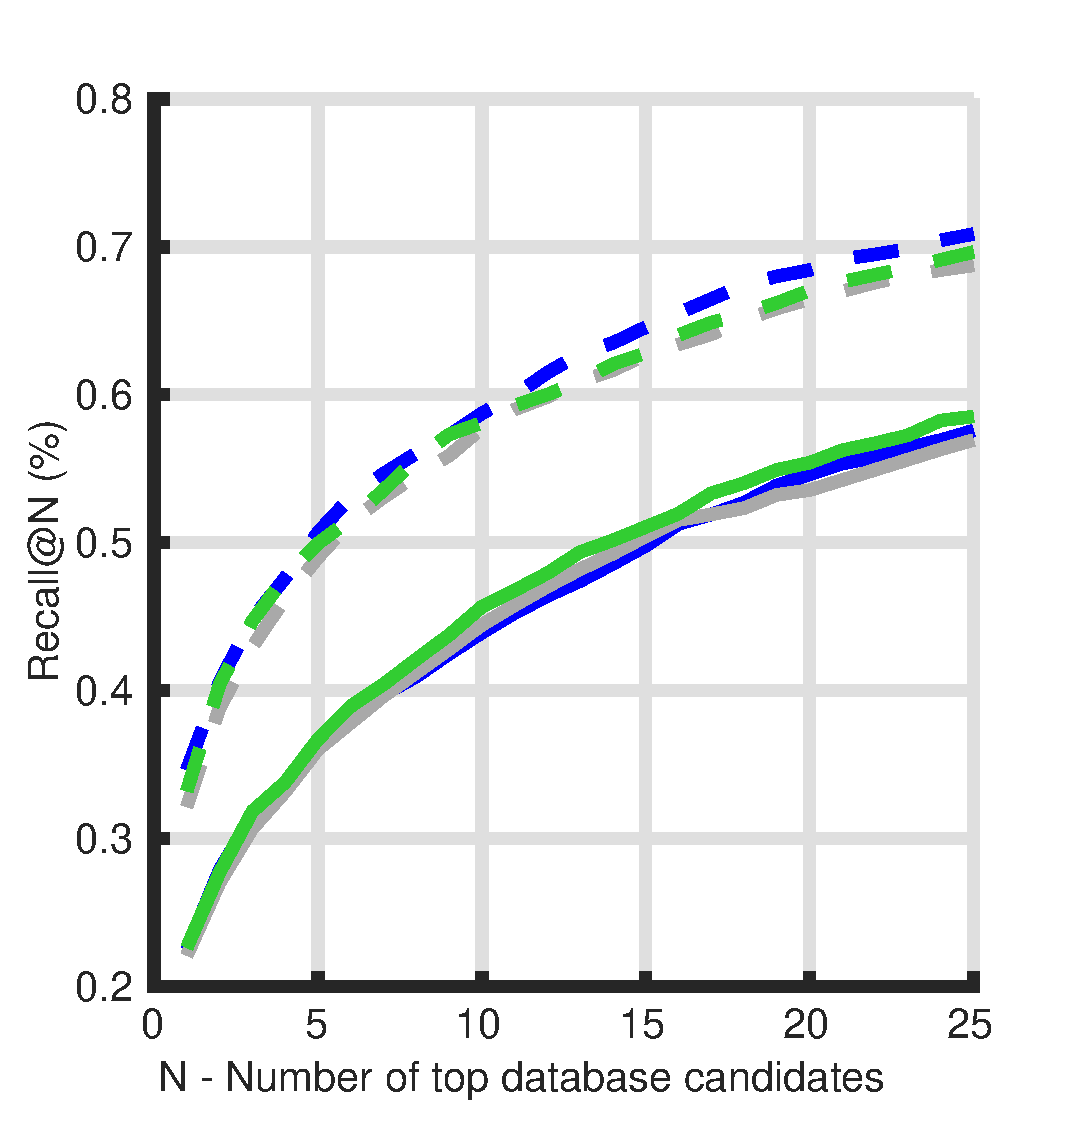
\includegraphics[width=\linewidth]{plot/depth_vs_ref/Results_cmu_snow/recall}
		
		d) CMU -- Snow
	\end{minipage}
	\begin{minipage}{0.27\linewidth}
		\center \scriptsize
		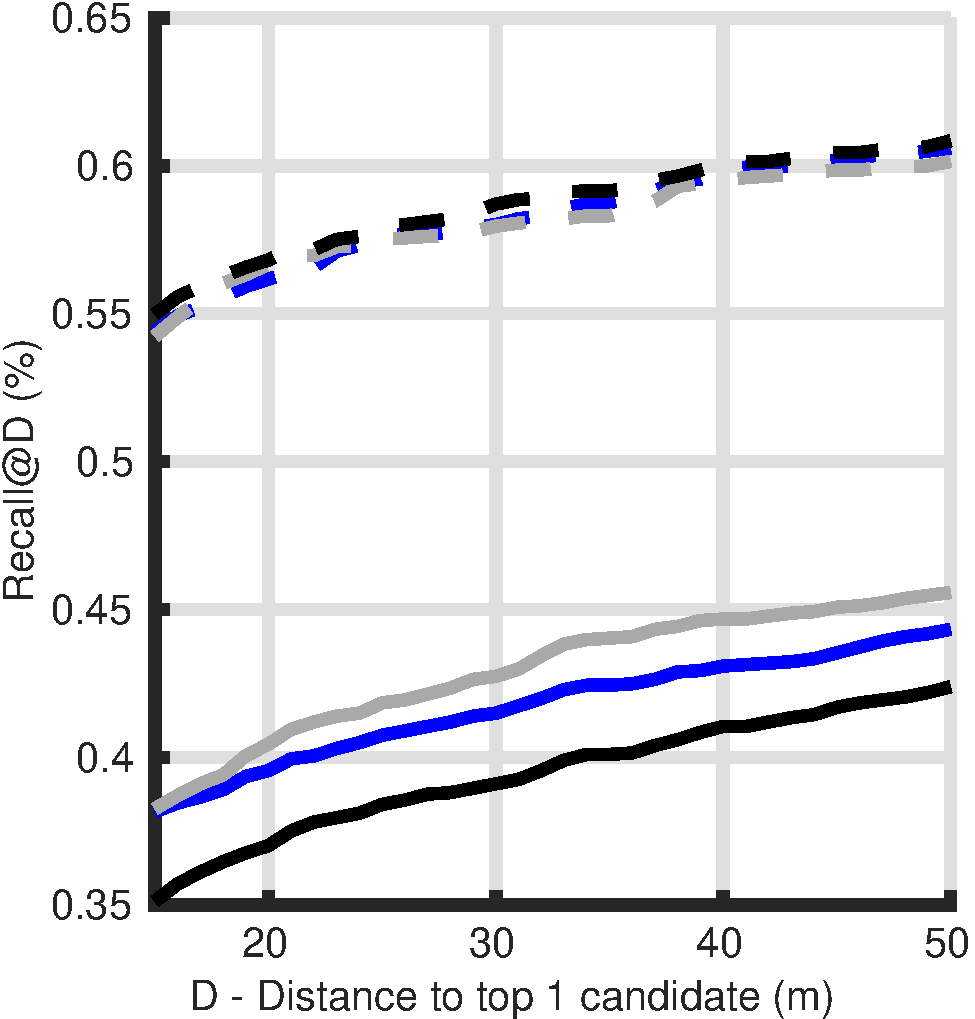
\includegraphics[width=\linewidth]{plot/depth_vs_ref/Results_cmu_autumn/distance}	
		
		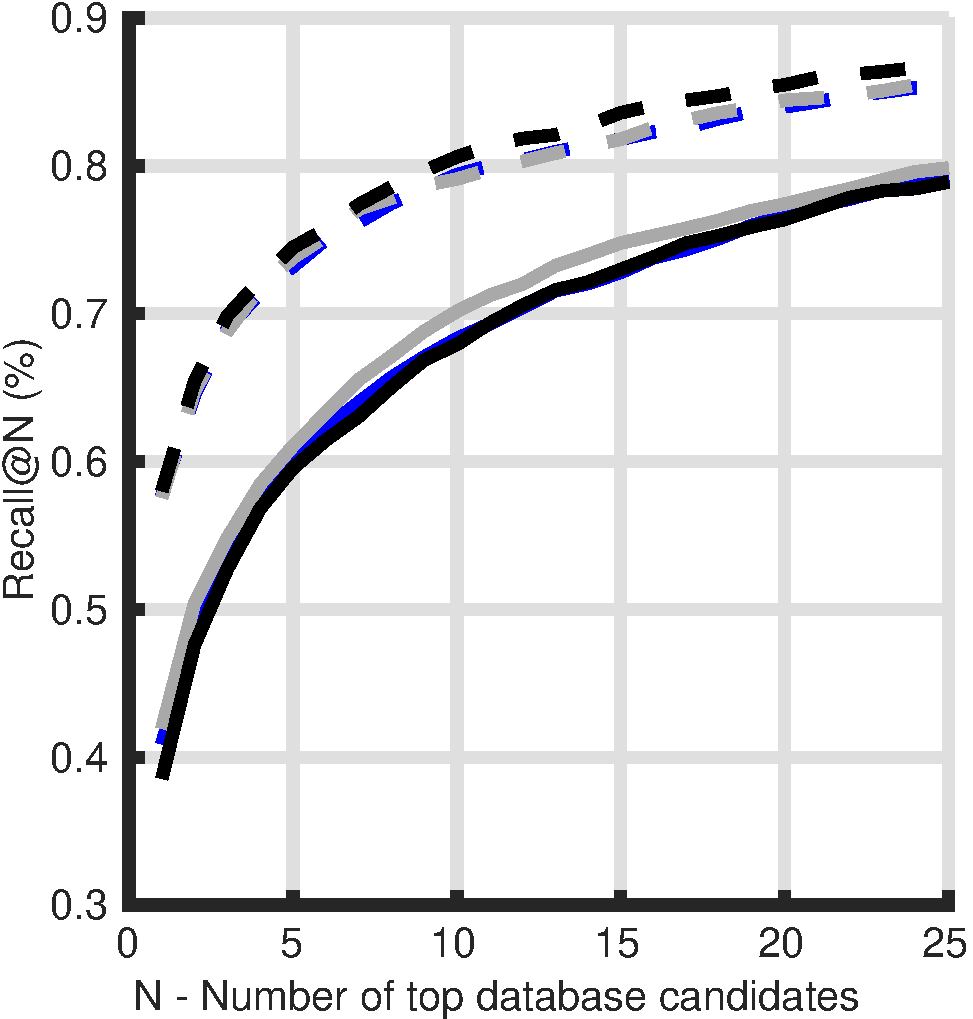
\includegraphics[width=\linewidth]{plot/depth_vs_ref/Results_cmu_autumn/recall}
		
		e) CMU -- Autumn
	\end{minipage}

	\vspace{5pt}	
	
	\begin{minipage}{0.27\linewidth}
		\center \scriptsize
		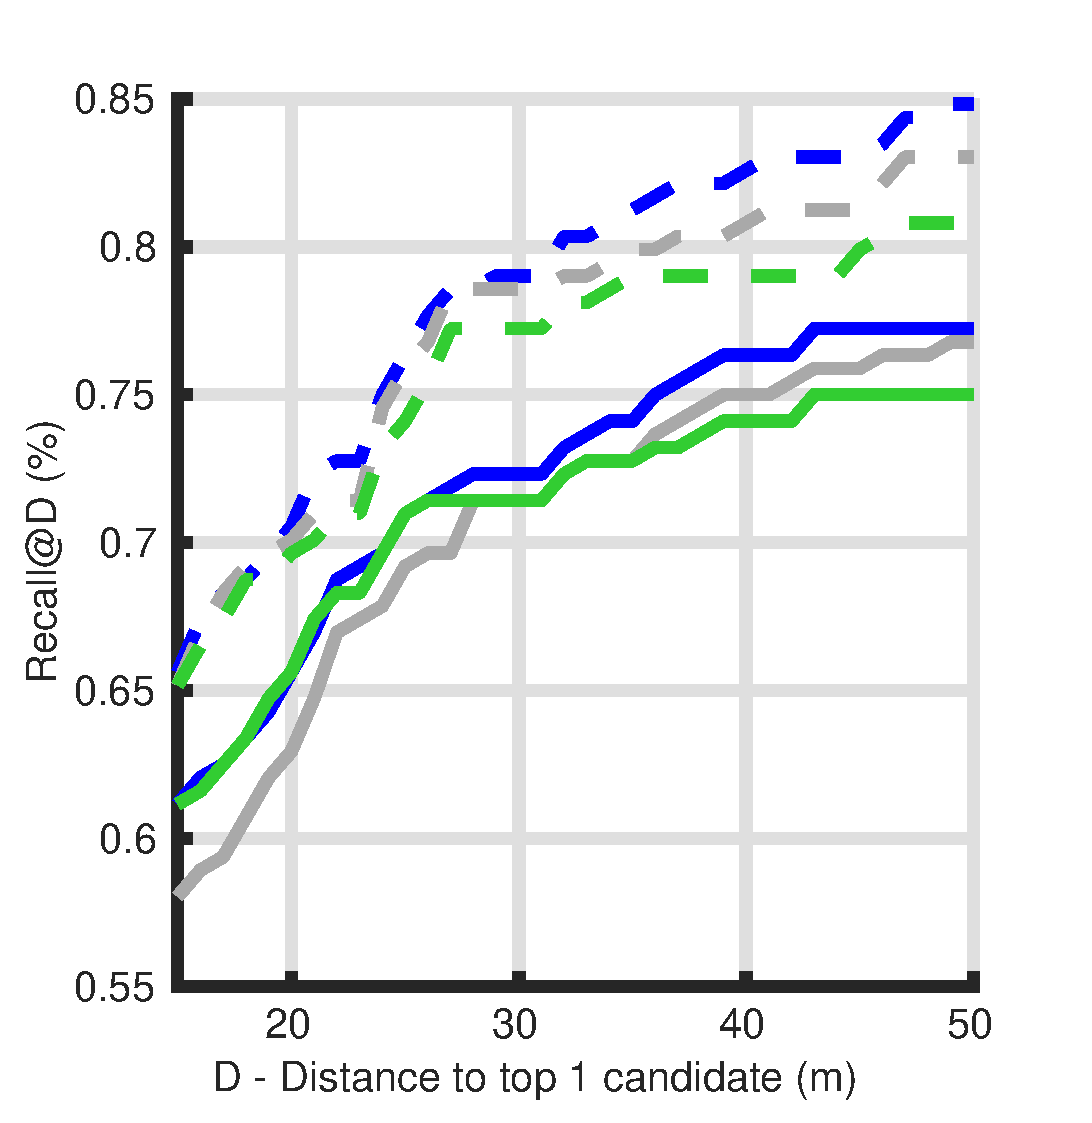
\includegraphics[width=\linewidth]{plot/depth_vs_ref/Results_lt_queries/distance}	
		
		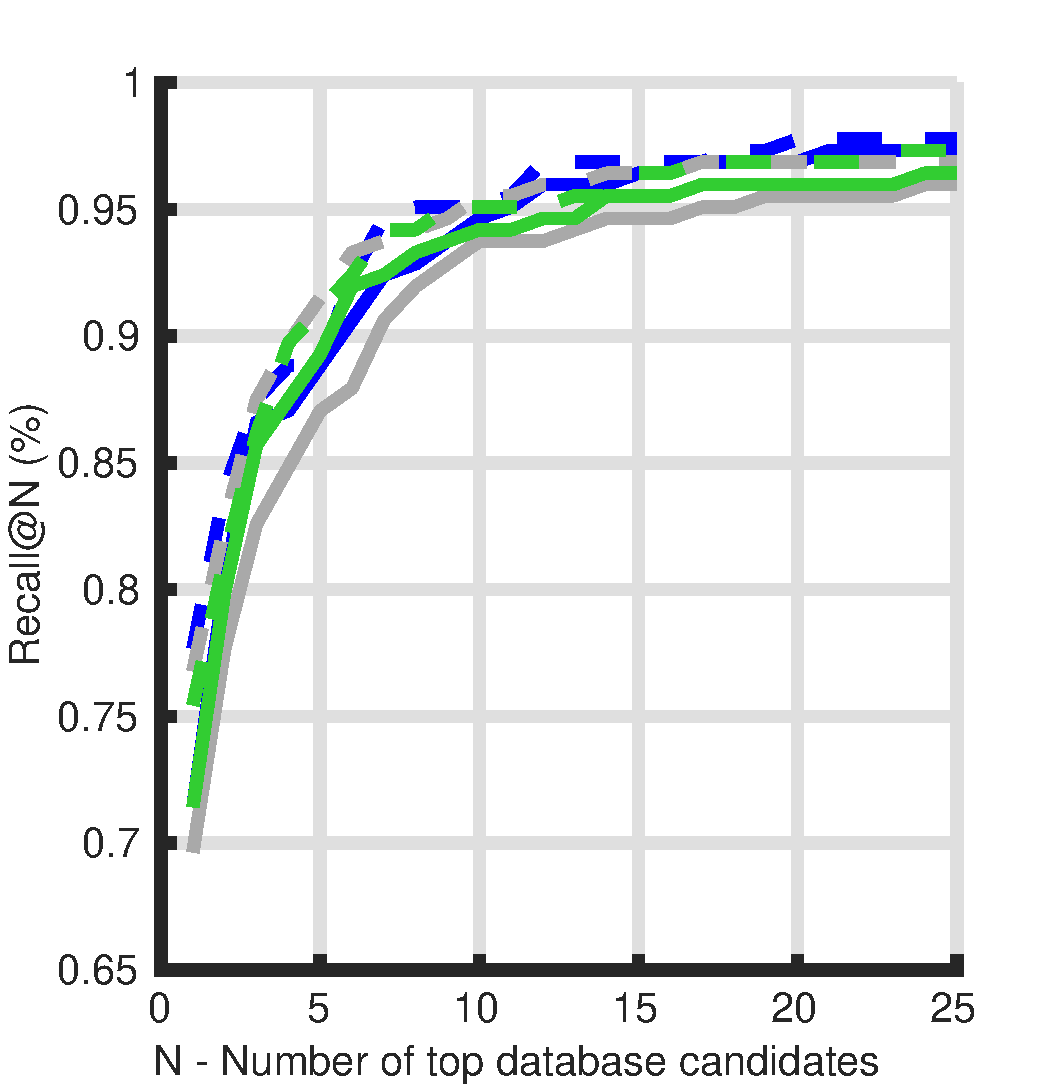
\includegraphics[width=\linewidth]{plot/depth_vs_ref/Results_lt_queries/recall}
		
		a) Oxford -- LT
	\end{minipage}
	\begin{minipage}{0.27\linewidth}
		\center \scriptsize
		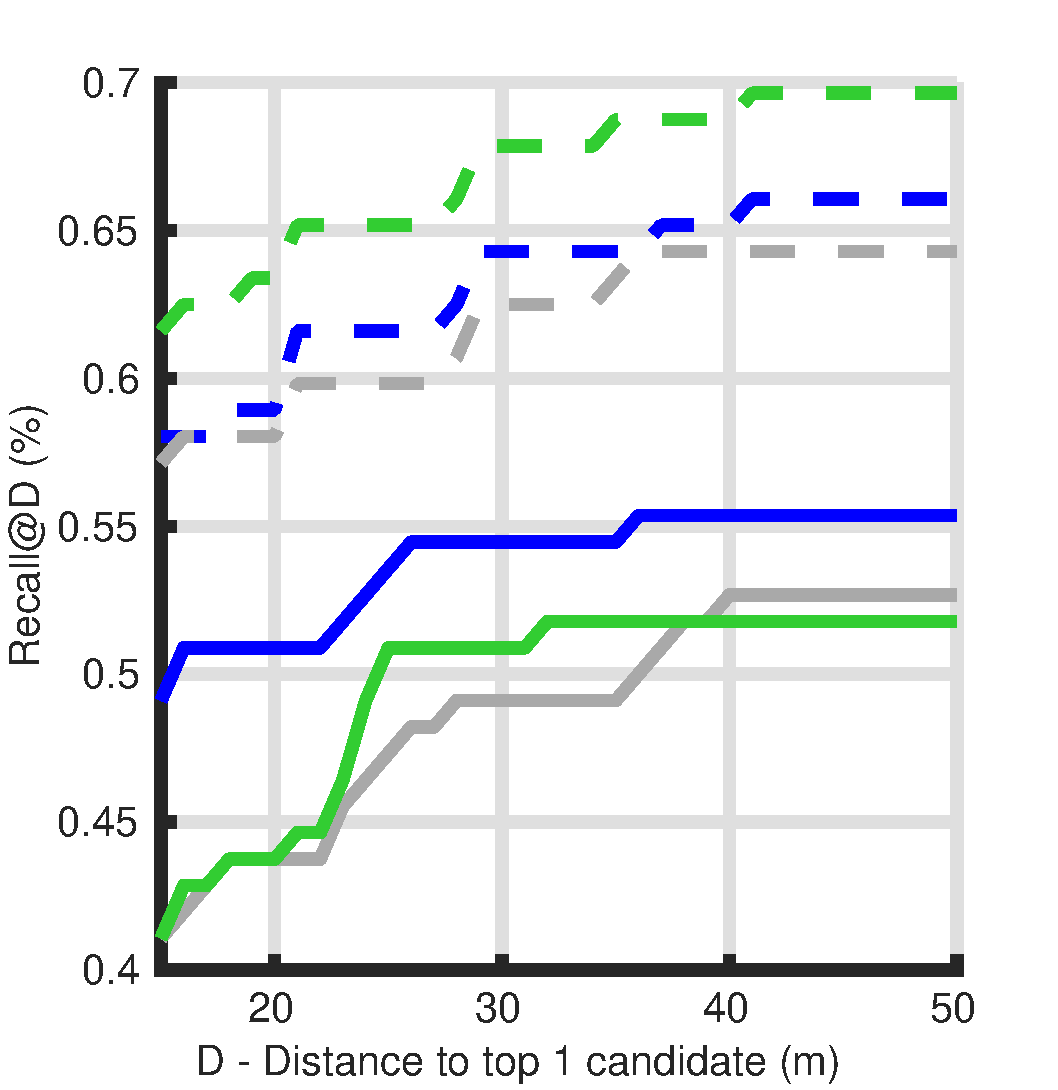
\includegraphics[width=\linewidth]{plot/depth_vs_ref/Results_snow_queries/distance}	
		
		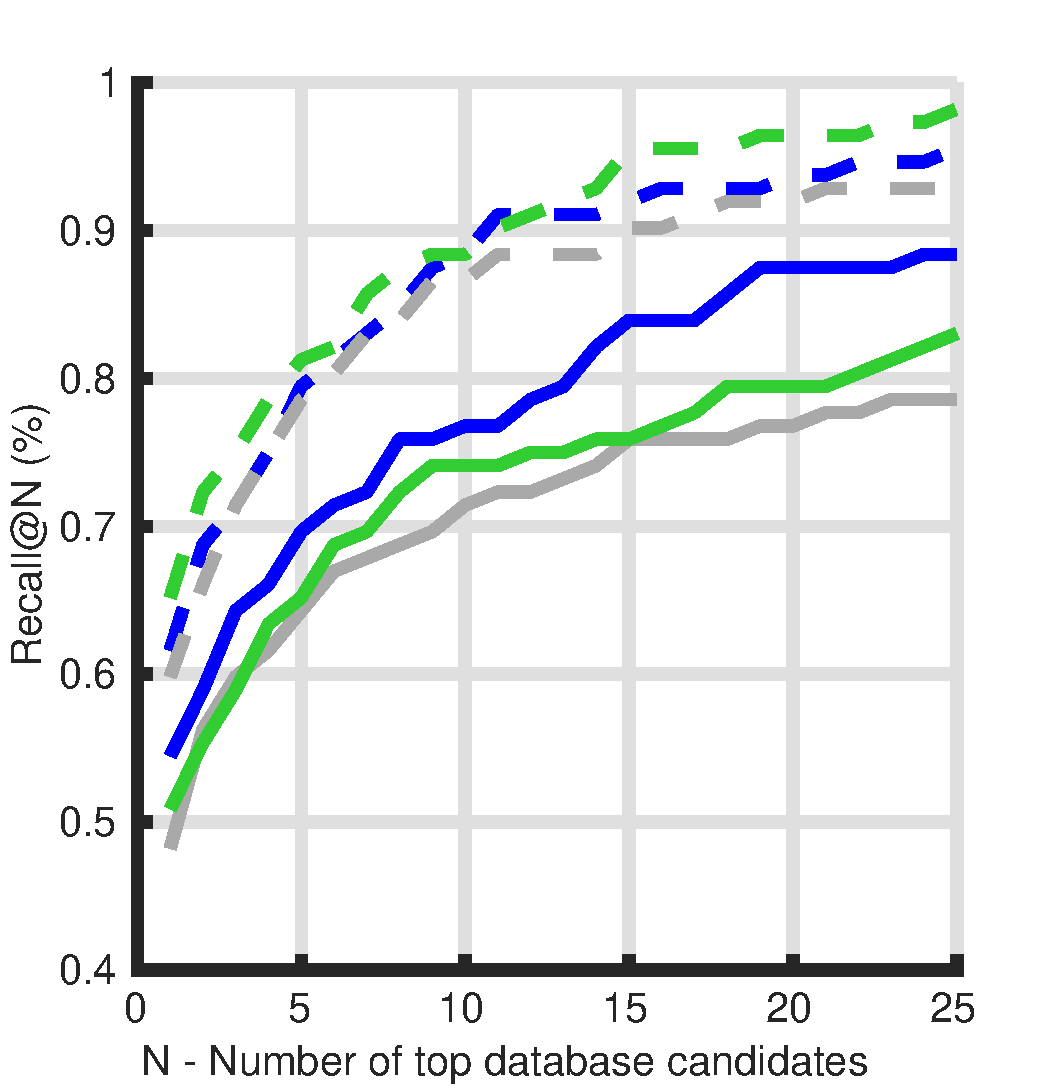
\includegraphics[width=\linewidth]{plot/depth_vs_ref/Results_snow_queries/recall}
				
		b) Oxford -- Snow
	\end{minipage}
	
	\vspace{0.2cm}
	
	\begin{scriptsize}
	\begin{tabular}{c l c l c l }
		\textcolor{blue}{\textbf{\Large{---}}} & Alexnet RGB(D) & 
		\textcolor{gray}{\textbf{\Large{---}}} & Alexnet RGB(R) &
		\textbf{\Large{---}} & Alexnet RGB(DR) \\
		\textcolor{blue}{\Large{- -}} & Resnet RGB(D) & 
		\textcolor{gray}{\Large{- -}} & Resnet RGB(R) & 
		\Large{- -} & Resnet RGB(DR) \\
	\end{tabular}		
	\end{scriptsize}

	\caption[Comparison of depth map and reflectance map as side information]{\label{fig:ref_vs_depth} \textbf{Comparison of depth map and reflectance map as side information.} The geometric information (\textcolor{blue}{in blue}) remains more informative than the reflectance map (\textcolor{gray}{in gray}) for the task of image description for localization. However, when combined (in \textcolor{lemon}{green}), depth map and reflectance map can benefit from each other and produce the most discriminative image descriptors for scenarios b, c \& e. Curves best viewed in colors.}
	
\end{figure}